\documentclass[class=NCU_thesis, crop=false]{standalone}
\begin{document}

\chapter{Event Selection}\label{Event selection}
	A number of selection is applied on the events in this study. Because the final state of the Z'-2HDM model contains no leptons (see fig. \ref{fig:zp2HDM}), one can define this zero-lepton region as the signal region (SR). However, there are other processes having the same final products as that of this model, which are recognized as the background. To further estimate the amount of the background events, one analyzes other processes that are similar to the background. These processes are called the control region (CR). Both SR and CR are discussed in this chapter. Some comparisons and characteristic selections of SR and CRs are summarized in table \ref{tab:SR vs CR}.

	\section{Signal Region}\label{SR}
		First, no baseline leptons candidates, including the $\tau$-leptons, are considered. The value of $E_T^{\mathrm{miss}}$ is required to be at least 150 GeV. Multijet backgrounds may pass the selection criteria. To further suppress this background, one adds two selections. The first one requires the azimuthal angle between $E_T^{\mathrm{miss}}$ and any of the three highest-$p_T$ jets ($\min(\Delta \phi(E_T^{\mathrm{miss}}, \mathrm{jet}))$) greater than 20$^\circ$. The forward jets are only considered if the number of central jets is less than 3. The other selection requires the azimuthal angle between $E_T^{\mathrm{miss}}$ and $p_T^{\mathrm{miss}}$ smaller than 90$^\circ$, where $p_T^{\mathrm{miss}}$ is the negative sum of object momentum measured by the inner detector.

		After these selections, one devides these events into two regions based on the value of $E_T^{\mathrm{miss}}$. Those whose $E_T^{\mathrm{miss}}$ is smaller than 500 GeV are defined as the resolved region, whilst the merged region contains those events with $E_T^{\mathrm{miss}}$ > 500 GeV. The resolved region is further divided into three regions, whose $E_T^{\mathrm{miss}}$ are within $\left(150, 200\right]$ GeV, $\left(200, 350\right]$ GeV, and $\left(350, 500\right]$ GeV. Different sets of selections are applied in these two regions and tabulated in table \ref{tab:resolved vs merged}.

		For the resolved region, the events are required to have at least two small-R jets, which is the reason of the naming of this region. In these jets, exactly two b-tagged jets are also required. The $p_T$ of one of the jets has to exceed 45 GeV. For the events with two (three or more) jets, the scalar sum of the $p_T$ of the highest two (three) jets is also required to be at least 120 (150) GeV. A requirement of $S_{\mathrm{object}} > 16$ is also applied. To further suppress the multijet backgrounds, a selection on the separation are required. Due to the conservation of the momentum, one expects the tracks of the $E_T^{\mathrm{miss}}$ and the Higgs candidate are back-to-back. The azimuthal angle between $E_T^{\mathrm{miss}}$ and the Higgs candidate is required to be greater than 120$^\circ$. The azimuthal angle between the two jets from the Higgs candidate ($\Delta \phi(\mathrm{jet}_1, \mathrm{jet}_2)$) tends to be large in multijet background events because of the topology. Thus, it is required to be smaller than 140$^\circ$ in this study. Furthermore, in order to reject $t\bar{t}$ background events, two more selections are added. One of them is $\Delta R(\mathrm{jet}_1, \mathrm{jet}_2) < 1.8$. The scalar sum of the first three highest $p_T$ of the jets is required to be greater than 63\% of the scalar sum of all jets is considered as the other one. At last, one adds a Higgs mass window selection on the two b-tagged jets, 50 GeV $< m_{\mathrm{jj}} <$ 280 GeV.
	
		As for the merged region, the events which contain at least one large-R jet are considered, which is the reason of the name "merged". The large-R (VR track) jet with the highest $p_T$ are referred to as the leading large-R (VR track) jet. Two leading VR track jets associated with the leading large-R jet are required be to b-tagged. Events with any VR track jets outside the large-R jets are rejected. To suppress the $t\bar{t}$ background events, the value of $p_T$ of the leading large-R jet is required to exceed 43\% of the scalar sum of the $p_T$ of the leading large-R jets and all small-R jets. Finally, the invariant mass of the large-R jet is also required to be within a Higgs mass window, 50 GeV $< m_{\mathrm{J}} <$ 270 GeV.
	
	\section{Control Region}
		Events containing leptons are used to define the CRs. One makes use of the CRs to estimate the main backgrounds of the Z'-2HDM model shown in fig. \ref{fig:zp2HDM}. These main backgrounds are shown in \ref{fig:background}. Based on the number of leptons of the analyzed events, they can be further categorized into two CRs. The $t\bar{t}$ and W+jets production are estimated from the 1-muon CR. The 2-lepton CR is used for the Z-jets events analyses.
	
		\begin{figure}[!hbt]
			%\captionsetup[subfigure]{labelformat=empty} % hide figure's number.
			\centering
			\subcaptionbox
			{\label{fig:subfig_ttbar}}
			{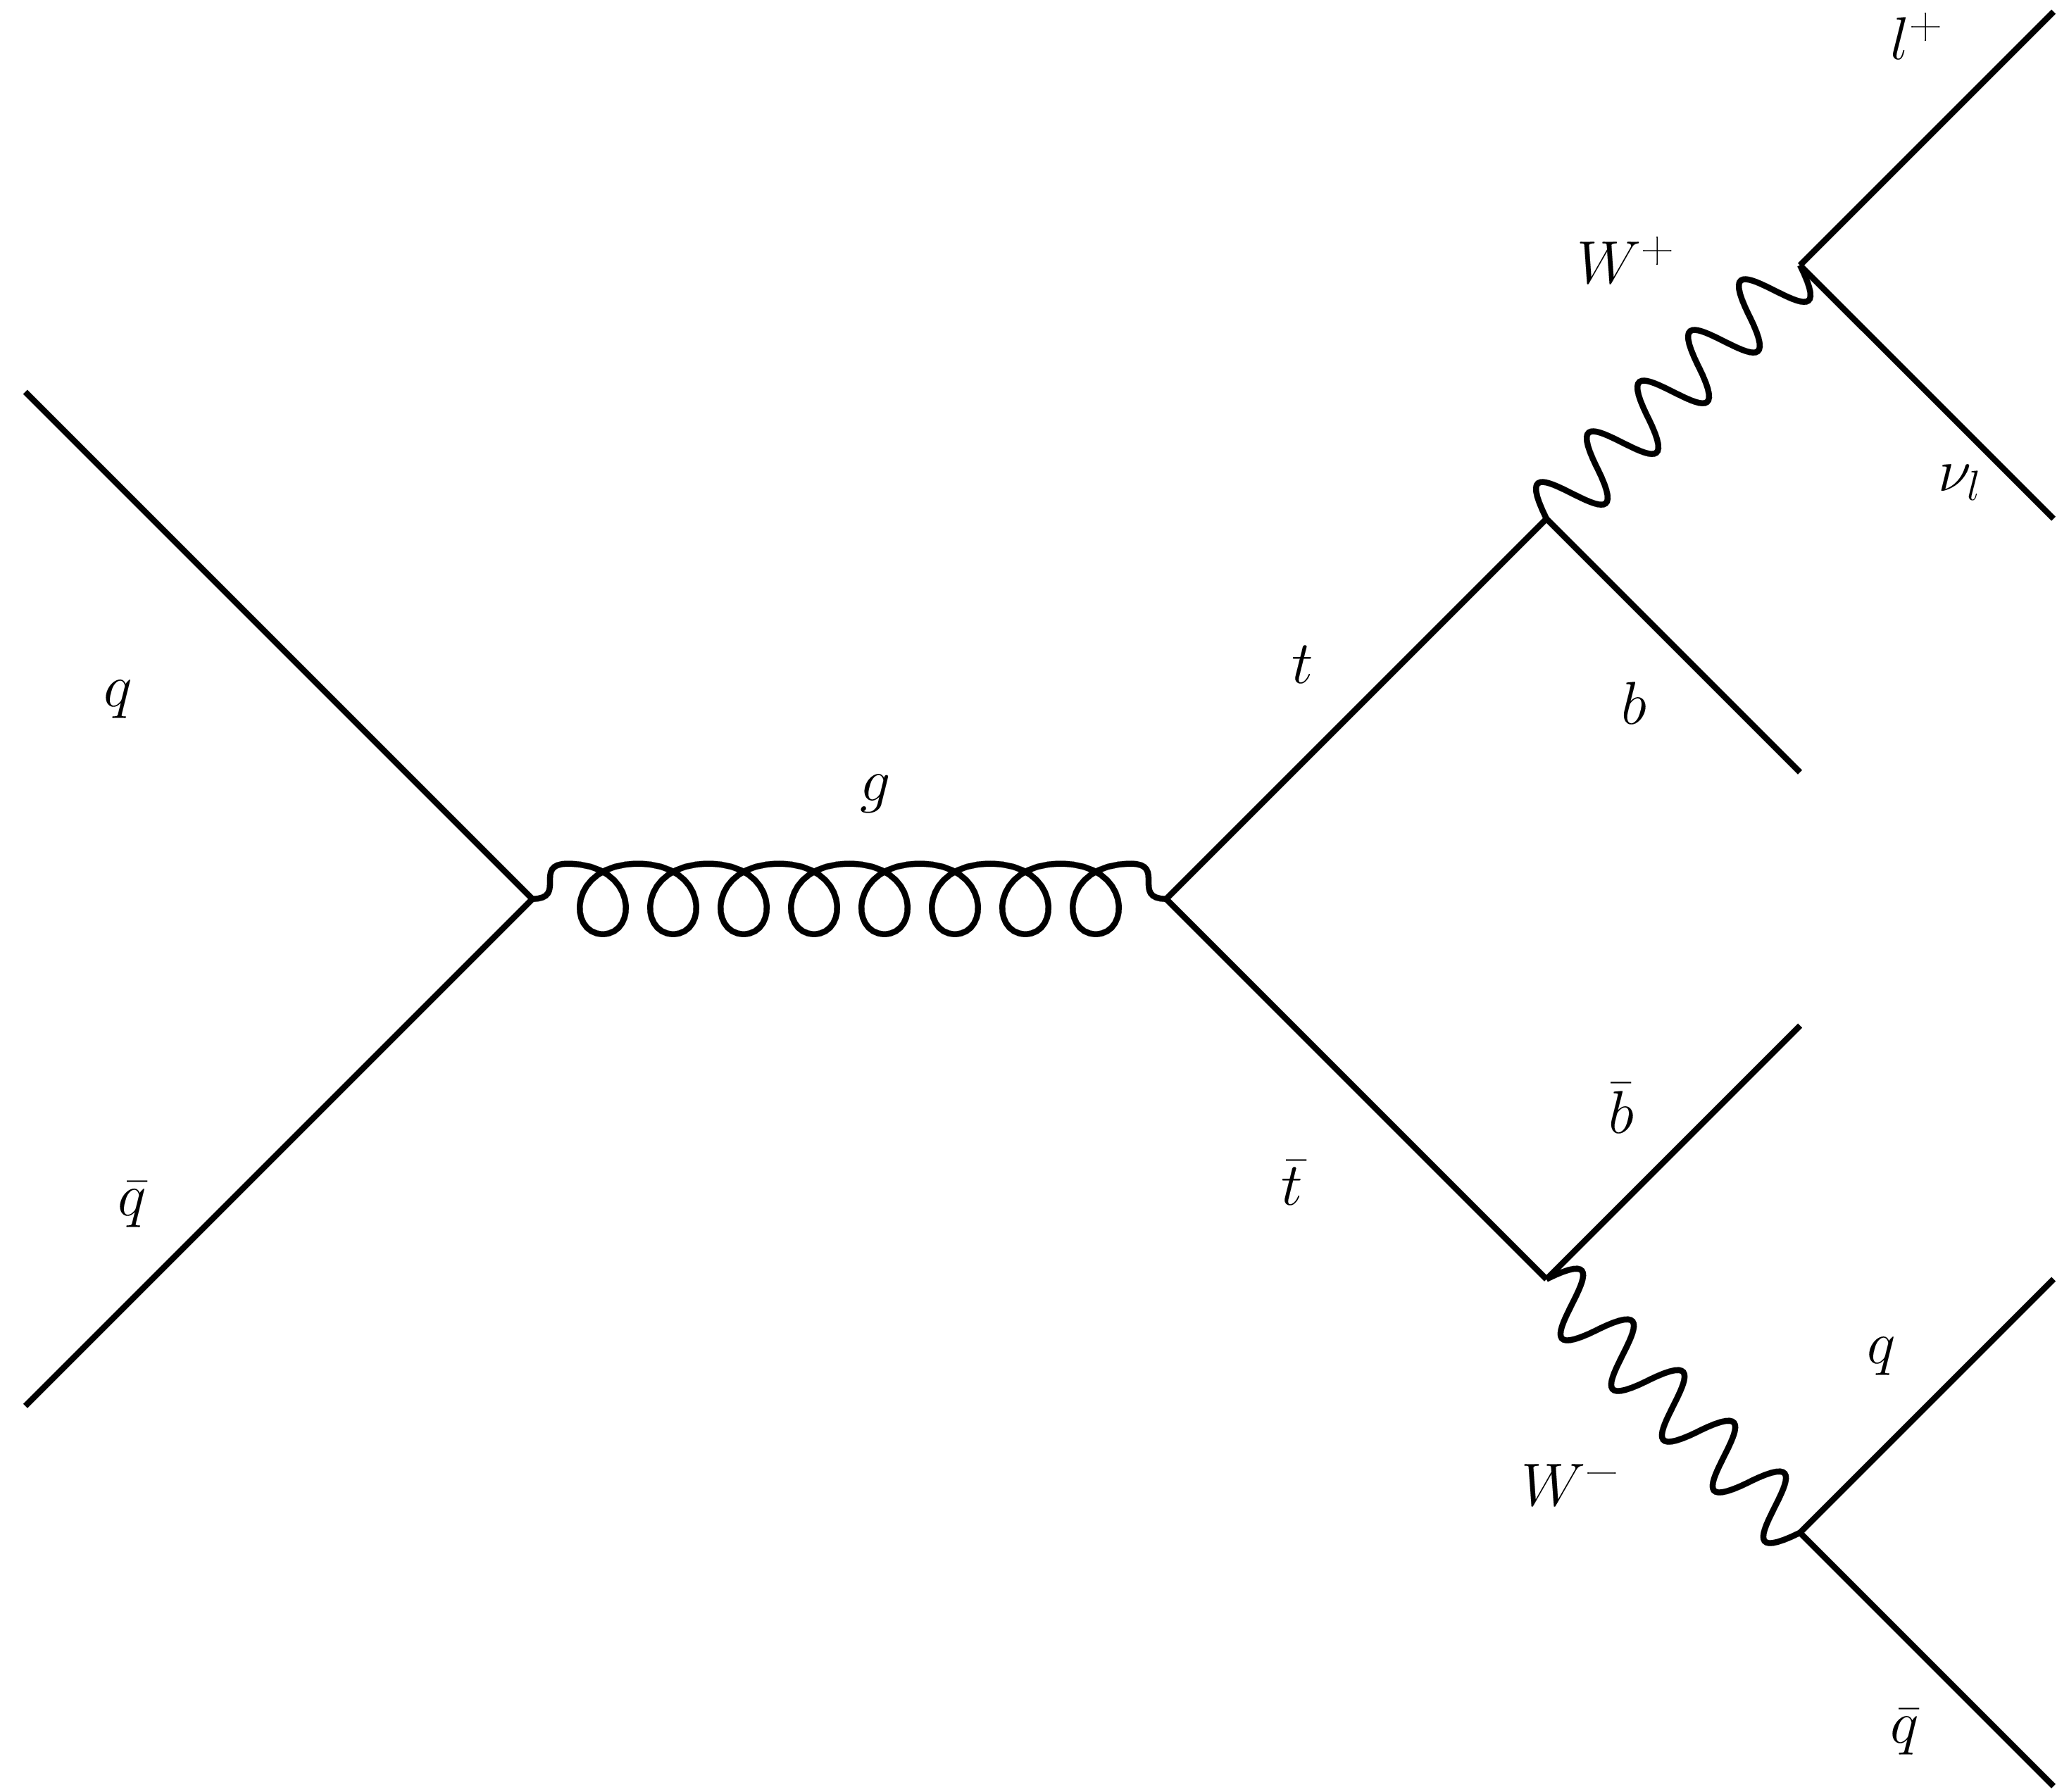
\includegraphics[width=0.3\linewidth]{ttbar.png}}
			~
			\subcaptionbox
			{\label{fig:subfig_Wjets}}
			{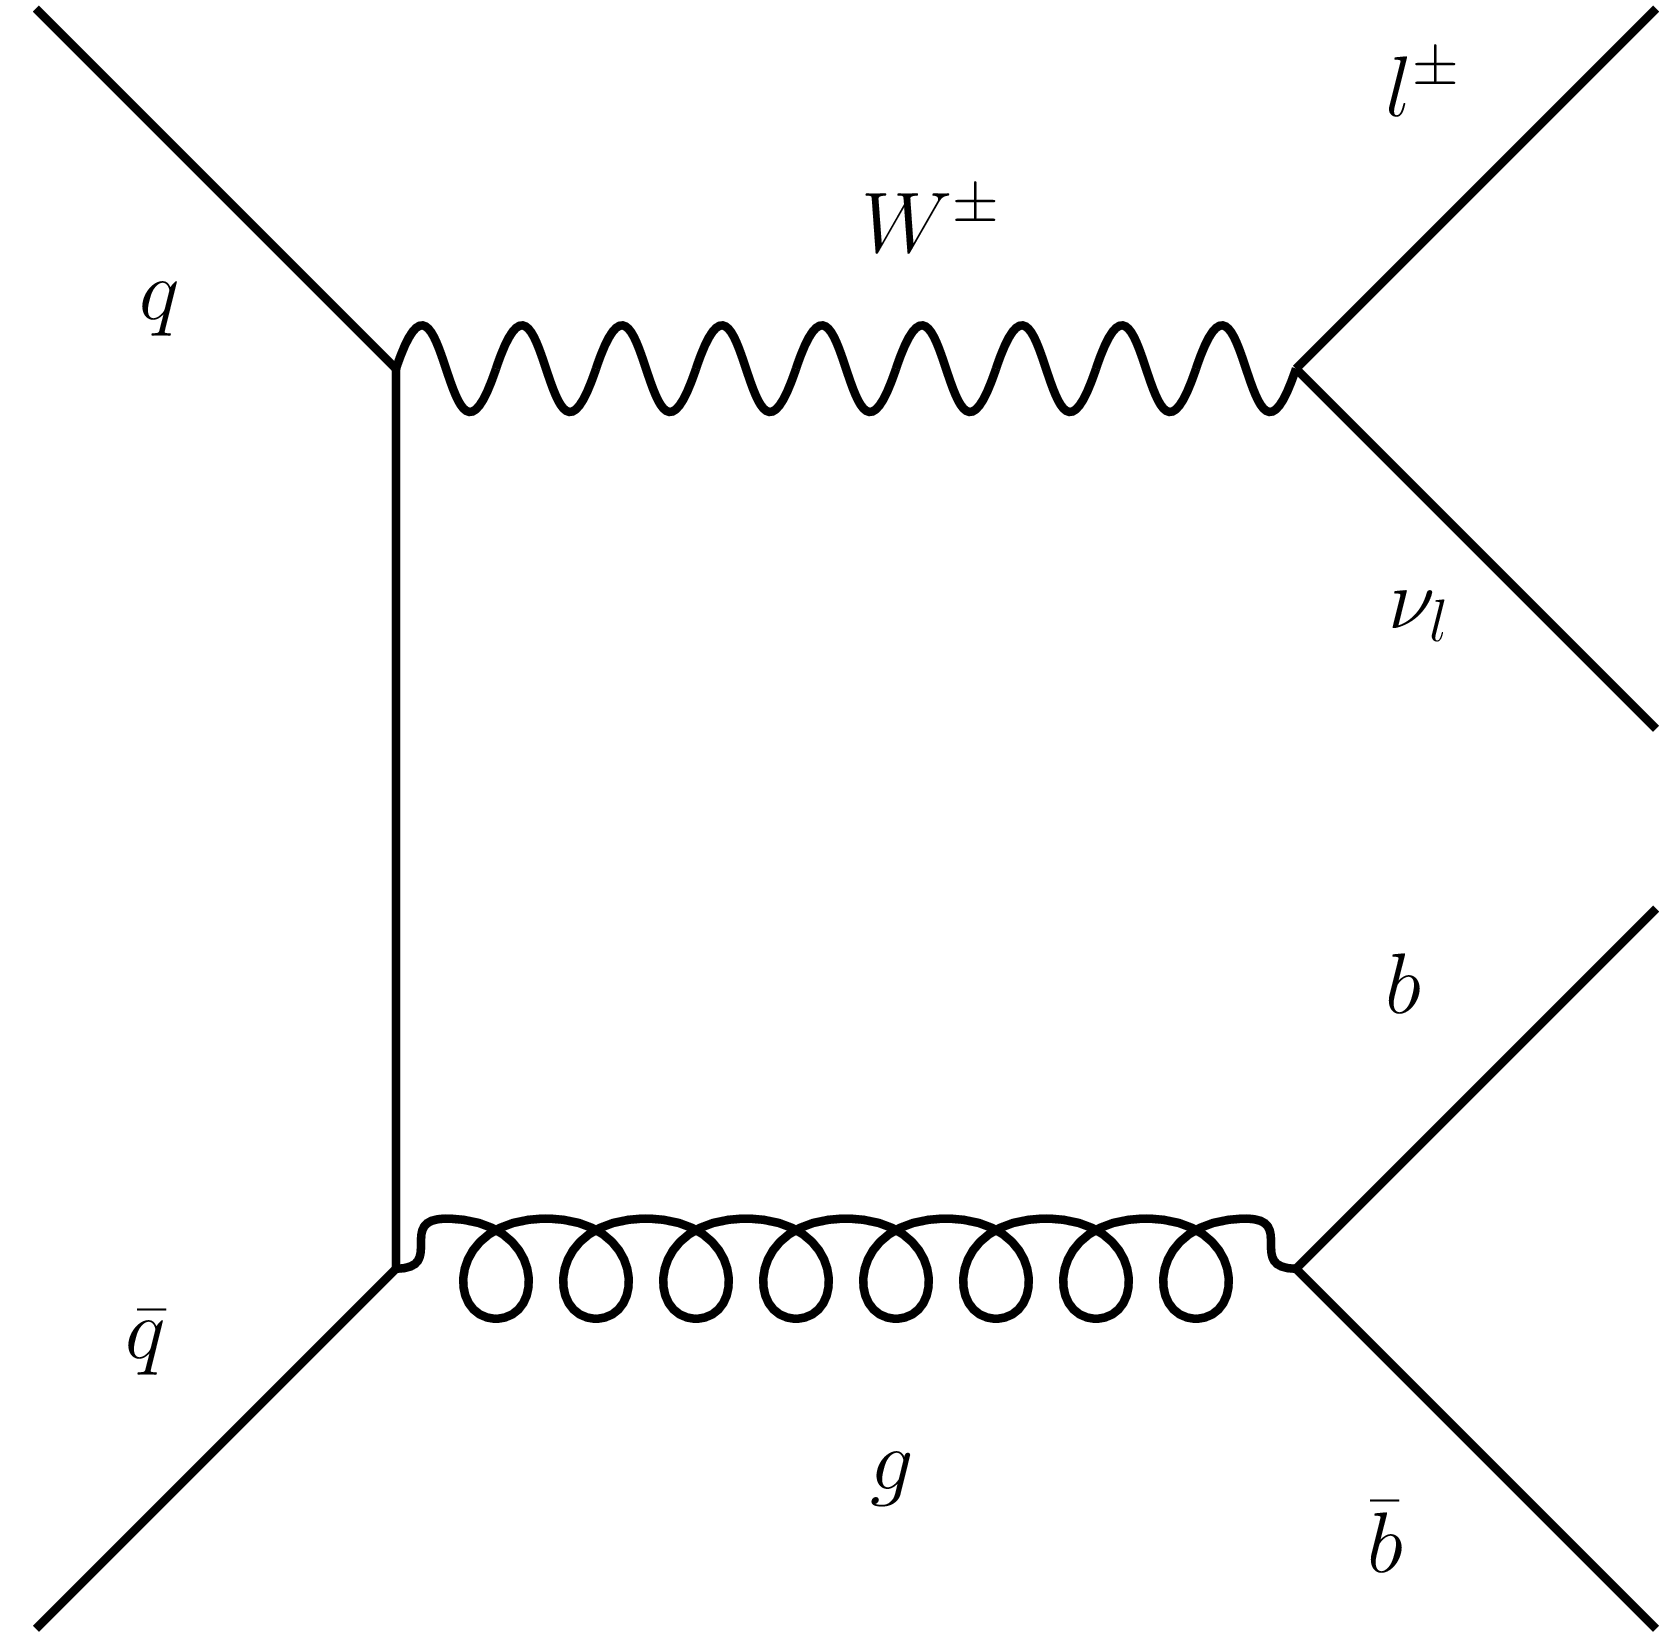
\includegraphics[width=0.3\linewidth]{Wjets.png}}
			%\vspace{\baselineskip} % 分隔上下列
			\subcaptionbox
			{\label{fig:subfig_Zjets}}
			{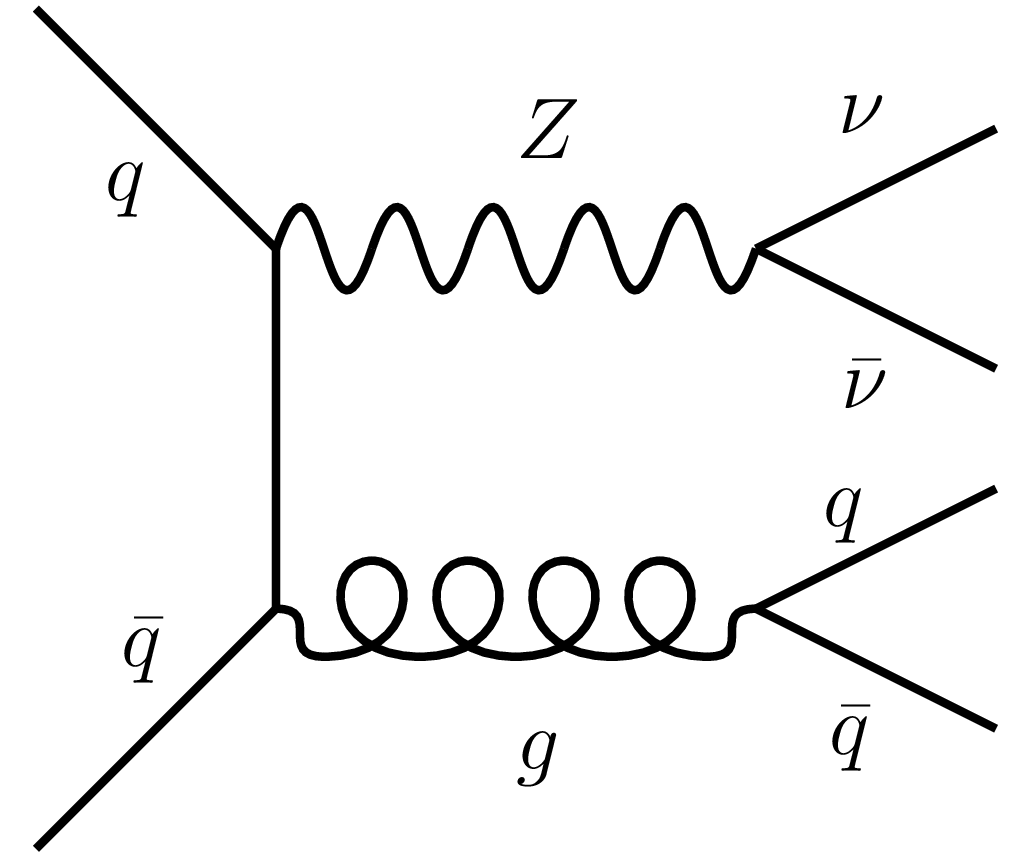
\includegraphics[width=0.3\linewidth]{Zjets.png}}
			\caption{The Feynamn diagram of the main background events of the Z'-2HDM model. From left to right, \subref{fig:subfig_ttbar} shows the $t\bar{t}$; \subref{fig:subfig_Wjets} shows the W+jets events; \subref{fig:subfig_Zjets} shows the Z+jets events. For the $t\bar{t}$ events, the lepton could also decay from the $\mathrm{W^-}$ boson, which is not shown in this figure.}
			\label{fig:background}
		\end{figure}

		\subsection{1-muon Control Region}
			Although there are leptons in figure \ref{fig:background} \subref{fig:subfig_ttbar} and \subref{fig:subfig_Wjets}, these events become the backgrounds because of misidentification or missed detections. As a result, the misidentified or undetected leptons would contribute to $E_T^{\mathrm{miss}}$. The 1-muon CR is made use of estimating the backgrounds of these $t\bar{t}$ and W+jets events.
	
			Because of the relatively higher fake rate of identification, single electron events are not considered in this background estimation. Therefore, no baseline electrons and exactly one signal muon are required. To mimic how these background events in SR behave, a "proxy" missing transverse momentum is defined as the sum of $E_T^{\mathrm{miss}}$ and the transverse momenta of the muon, or $E_T^{\mathrm{miss, no}\ \mu}$. The resolved and merged region are also defined using the threshold of 500 GeV on $E_T^{\mathrm{miss, no }\ \mu}$. Other selections are the same as those mentioned in section \ref{SR} except the $S_{\mathrm{object}}$ selection in the resolved region.
	
		\subsection{2-lepton Control Region}\label{2LCR}
			The neutrinos in figure \ref{fig:background} \subref{fig:subfig_Zjets} cannot be detected and thus are part of the contributions to $E_T^{\mathrm{miss}}$. The 2-lepton CR serves as the estimation of this background.
		
			Two same-flavor leptons are required first. For both two-electron or two-muon cases, one lepton is required to be the signal one while the other has to pass the criteria of the baseline ones. Additional requirement for the two-muon case is to have opposite charge. In order to make sure that the lepton pair truly decay from the Z boson candidate, a dilepton mass window is applied. The requirement on invariant mass of the two-electron (muon) system is 83 GeV $< m_{\mathrm{ee}} <$ 99 GeV (71 GeV $< m_{\mathrm{\mu \mu}} <$ 106 GeV). The "proxy" missing transverse momentum is the absoulte value of the sum of the transverse momentum of the two-leptons, or $p_T^{ll}$. One makes use of $p_T^{ll}$ to define the resolved merged region based on the 500 GeV boundary. Those selections stated in section \ref{SR} except the $S_{\mathrm{object}}$ selection in the resolved region are applied. Apart from that, in order to reduce the $t\bar{t}$ and single top background in this CR, the $S_{\mathrm{event}}$ is required to be less than 3.5 $\mathrm{GeV}^\frac{1}{2}$.
		
			\begin{table}[h]
				%\centering
				\caption{Comparison of signal region and two control regions. This table only shows the characteristic selections and different definitions of (proxy) missing transverse momentum in different regions. One should combine the selections summarized in table \ref{tab:resolved vs merged} to get the whole set of selections in a certain region.}
				\label{tab:SR vs CR}
				\begin{tabular}{|c|c|c|c|}
					\hline
					region & signal region & 1-muon control region & 2-lepton control region\\
					\hline
					lepton selection & no loose leptons & \shortstack{one signal muon\\no baseline electrons} & \shortstack{two baseline muons or electrons\\one of them being signal}\\
					\hline
					\shortstack{(proxy) missing\\transverse momentum} & $E_T^{\mathrm{miss}}$ & $E_T^{\mathrm{miss, no}\ \mu} = E_T^{\mathrm{miss}} + p_T^\mu$ & $p_T^{ll}$\\
					\hline
					\shortstack{$E_T^{\mathrm{miss}}$ significance\\selection (resolved only)} & $S_{\mathrm{object}} > 16$ & - & $S_{\mathrm{event}} <$ 3.5 $\mathrm{GeV}^\frac{1}{2}$\\
					\hline
					additional & - & - & \shortstack{83(99) GeV $< m_{\mathrm{ee\left(\mu \mu\right)}} <$ 99(106) GeV\\opposite muon charge}\\
					\hline
				\end{tabular}
			\end{table}
		
			\begin{table}[h]
				%\centering
				\caption{Summary of common selections of resolved and merged region for all SR and CRs. One should combine the characteristic selections stated in \ref{tab:SR vs CR} to get the whole set of selections in a certain region.}
				\label{tab:resolved vs merged}
				\begin{tabular}{|c|c|}
					\hline
					resolved & merged\\
					\hline
					\multicolumn{2}{|c|}{$\tau$-veto}\\
					\hline
					\multicolumn{2}{|c|}{$\min (\Delta \phi(E_T^{\mathrm{miss}}, \mathrm{jet})) > 20^\circ$}\\
					\hline
					\multicolumn{2}{|c|}{$\Delta \phi(E_T^{\mathrm{miss}}, p_T^{\mathrm{miss}}) < 90^\circ$}\\
					\hline
					(proxy) $E_T^{\mathrm{miss}} \in \left(150, 500\right]$ GeV & (proxy) $E_T^{\mathrm{miss}} \in \left(500, \infty \right)$ GeV\\
					\hline
					$\geq$ 2 b-tagged small-R jets & $\geq$ 1 large-R jet\\
					\hline
					$\Delta R(\mathrm{jet_1}, \mathrm{jet_2}) < 1.8$ & $\Delta R(\mathrm{VR_1}, \mathrm{VR_2}) > R_{\mathrm{min}}$\\
					\hline
					$p_T^{\mathrm{jet_1}} > 45$ GeV or $p_T^{\mathrm{jet_2}} > 45$ GeV & -\\
					\hline
					$\sum_{i=1}^{2(3)} p_T^{\mathrm{jet}_i} >$ 120(150) GeV & - \\
					\hline
					$\Delta \phi(E_T^{\mathrm{miss}}, h) > 120^\circ$ & -\\
					\hline
					$\Delta \phi(\mathrm{jet}_1, \mathrm{jet}_2) < 140^\circ$ & -\\
					\hline
					$\sum_{i=1}^{3} p_T^{\mathrm{jet}_i} / \sum_{i=1}^{\infty} p_T^{\mathrm{jet}_i} > 0.63$ & $p_T^{\mathrm{large-R jet}} / (p_T^{\mathrm{large-R \ jet}} + \sum p_T^{\mathrm{small-R \ jet}}) > 0.43$\\
					\hline
					50 GeV $< m_{\mathrm{jj}} <$ 280 GeV & 50 GeV $< m_{\mathrm{J}} <$ 270 GeV\\
					\hline
				\end{tabular}
			\end{table}

\end{document}